% Options for packages loaded elsewhere
\PassOptionsToPackage{unicode}{hyperref}
\PassOptionsToPackage{hyphens}{url}
%
\documentclass[
  10pt,
  ignorenonframetext,
]{beamer}
\usepackage{pgfpages}
\setbeamertemplate{caption}[numbered]
\setbeamertemplate{caption label separator}{: }
\setbeamercolor{caption name}{fg=normal text.fg}
\beamertemplatenavigationsymbolsempty
% Prevent slide breaks in the middle of a paragraph
\widowpenalties 1 10000
\raggedbottom
\setbeamertemplate{part page}{
  \centering
  \begin{beamercolorbox}[sep=16pt,center]{part title}
    \usebeamerfont{part title}\insertpart\par
  \end{beamercolorbox}
}
\setbeamertemplate{section page}{
  \centering
  \begin{beamercolorbox}[sep=12pt,center]{part title}
    \usebeamerfont{section title}\insertsection\par
  \end{beamercolorbox}
}
\setbeamertemplate{subsection page}{
  \centering
  \begin{beamercolorbox}[sep=8pt,center]{part title}
    \usebeamerfont{subsection title}\insertsubsection\par
  \end{beamercolorbox}
}
\AtBeginPart{
  \frame{\partpage}
}
\AtBeginSection{
  \ifbibliography
  \else
    \frame{\sectionpage}
  \fi
}
\AtBeginSubsection{
  \frame{\subsectionpage}
}
\usepackage{amsmath,amssymb}
\usepackage{lmodern}
\usepackage{ifxetex,ifluatex}
\ifnum 0\ifxetex 1\fi\ifluatex 1\fi=0 % if pdftex
  \usepackage[T1]{fontenc}
  \usepackage[utf8]{inputenc}
  \usepackage{textcomp} % provide euro and other symbols
\else % if luatex or xetex
  \usepackage{unicode-math}
  \defaultfontfeatures{Scale=MatchLowercase}
  \defaultfontfeatures[\rmfamily]{Ligatures=TeX,Scale=1}
\fi
% Use upquote if available, for straight quotes in verbatim environments
\IfFileExists{upquote.sty}{\usepackage{upquote}}{}
\IfFileExists{microtype.sty}{% use microtype if available
  \usepackage[]{microtype}
  \UseMicrotypeSet[protrusion]{basicmath} % disable protrusion for tt fonts
}{}
\makeatletter
\@ifundefined{KOMAClassName}{% if non-KOMA class
  \IfFileExists{parskip.sty}{%
    \usepackage{parskip}
  }{% else
    \setlength{\parindent}{0pt}
    \setlength{\parskip}{6pt plus 2pt minus 1pt}}
}{% if KOMA class
  \KOMAoptions{parskip=half}}
\makeatother
\usepackage{xcolor}
\IfFileExists{xurl.sty}{\usepackage{xurl}}{} % add URL line breaks if available
\IfFileExists{bookmark.sty}{\usepackage{bookmark}}{\usepackage{hyperref}}
\hypersetup{
  pdftitle={Introductory Statistics for Economics},
  pdfauthor={Duong Trinh},
  hidelinks,
  pdfcreator={LaTeX via pandoc}}
\urlstyle{same} % disable monospaced font for URLs
\newif\ifbibliography
\setlength{\emergencystretch}{3em} % prevent overfull lines
\providecommand{\tightlist}{%
  \setlength{\itemsep}{0pt}\setlength{\parskip}{0pt}}
\setcounter{secnumdepth}{-\maxdimen} % remove section numbering
\ifluatex
  \usepackage{selnolig}  % disable illegal ligatures
\fi

\title{Introductory Statistics for Economics}
\subtitle{ECON1013: TUTORIAL 4}
\author{Duong Trinh}
\date{March 2022}
\institute{University of Glasgow}

\begin{document}
\frame{\titlepage}

\begin{frame}{Exercise 1}
\protect\hypertarget{exercise-1}{}
As part of a ``Math for the Twenty-First Century'' initiative, Bayview
High was chosen to participate in the evaluation of a new algebra and
geometry curriculum. In the recent past, Bayview's students were
considered ``typical'', having earned scores on standardized exams that
were very consistent with national averages.

Two years ago, a cohort of 86 Bayview students, all randomly selected,
were assigned to a special set of classes that integrated algebra and
geometry. According to test results that have just been released, those
students averaged 502 on the math exam, and nationwide seniors averaged
494 with a standard deviation of 124.

\begin{enumerate}
  \item [(a)] Can it be claimed at $5\%$ significance level that the new curriculum had effect? Justify your answer.
  \item [(b)] Compute the p-value associated with the test statistics. How should it be interpreted? 
\end{enumerate}
\end{frame}

\begin{frame}{(a) Hypothesis Testing with \(\alpha = 0.05\)}
\protect\hypertarget{a-hypothesis-testing-with-alpha-0.05}{}
Procedure includes 4 steps: \vspace{1.5mm}

\begin{itemize}
    \item Null hypothesis $H_0$
    \vspace{1.5mm}
    \item Alternative hypothesis $H_1$
    \vspace{1.5mm}
    \item Decision rule
    \vspace{1.5mm}
    \item Conclusion
\end{itemize}
\end{frame}

\begin{frame}{(a) Hypothesis Testing with \(\alpha = 0.05\)}
\protect\hypertarget{a-hypothesis-testing-with-alpha-0.05-1}{}
Denote \(\mu\) the true mean of math score if students paticipated in
the new curriculum.\\

\begin{itemize}
    \item Null hypothesis $H_0$
        \begin{itemize}
            \item [$\square$] $H_0$: The new curriculum had no effect\\
                  $H_0: \mu = 494$
    \end{itemize}
    \vspace{1.5mm}
    \item Alternative hypothesis $H_1$
        \begin{itemize}
            \item [$\square$] $H_1$: The new curriculum had effect\\
                  $H_1: \mu \neq 494$
        \end{itemize}
    \vspace{1.5mm}
    \item Decision rule
    \vspace{1.5mm}
    \item Conclusion
\end{itemize}
\end{frame}

\begin{frame}{(a) Hypothesis Testing with \(\alpha = 0.05\)}
\protect\hypertarget{a-hypothesis-testing-with-alpha-0.05-2}{}
Denote \(\mu\) the true mean of math score if students paticipated in
the new curriculum.\\

\begin{itemize}
    \item Null hypothesis $H_0$
        \begin{itemize}
            \item [$\square$] $H_0$: The new curriculum had no effect\\
                  $H_0: \mu = 494$
    \end{itemize}
    \vspace{1.5mm}
    \item Alternative hypothesis $H_1$
        \begin{itemize}
            \item [$\square$] $H_1$: The new curriculum had effect\\
                  $H_1: \mu \neq 494$\\
        \end{itemize}
        $\Longrightarrow$ This is an \textit{two-tail test}
    \vspace{1.5mm}
    \item Decision rule
    \vspace{1.5mm}
    \item Conclusion
\end{itemize}
\end{frame}

\begin{frame}{Decision Rule}
\protect\hypertarget{decision-rule}{}
Given the sample size and the sampling scheme, the sample average is
asymptotically normally distributed: \[
\frac{\bar{X} - \mu_0}{\sigma/\sqrt{n}} \sim N(0,1)
\]

\begin{figure}
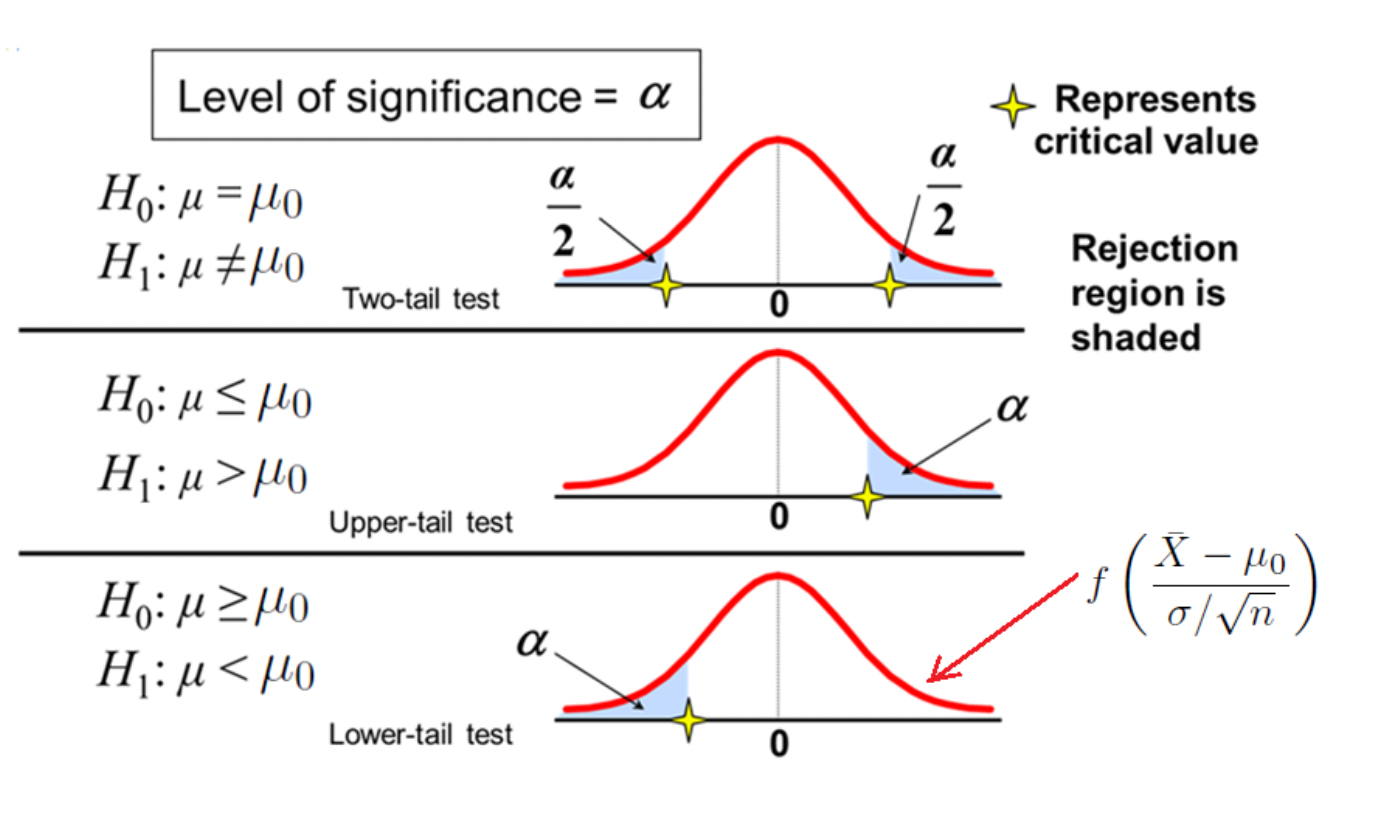
\includegraphics[width=0.8\linewidth]{/Users/duongtrinh/Dropbox/GLASGOW/GTA/ECON1013/Tutorials/Tutorial 4/Decision Rule} \caption{Level of Significance and the Rejection Region: one-sided vs two-sided alternatives}\label{fig:unnamed-chunk-1}
\end{figure}
\end{frame}

\begin{frame}{Decision Rule}
\protect\hypertarget{decision-rule-1}{}
For two-sided test, reject \(H_0\) if: \[
z = \frac{\bar{x}-\mu_0}{\sigma/\sqrt{n}} < - z_{\frac{\alpha}{2}} \text{ or } z = \frac{\bar{x}-\mu_0}{\sigma/\sqrt{n}} > z_{\frac{\alpha}{2}}
\] Notice that: \[
z = \frac{\bar{x}-\mu_0}{\sigma/\sqrt{n}} = \frac{502 - 494}{124/\sqrt{86}} \approx 0.5983 
\] and \(z_{\frac{\alpha}{2}} = z_{0.025} = 1.96\)
\end{frame}

\begin{frame}{(a) Hypothesis Testing with \(\alpha = 0.05\)}
\protect\hypertarget{a-hypothesis-testing-with-alpha-0.05-3}{}
Denote \(\mu\) the true mean of math score if students paticipated in
the new curriculum.\\

\begin{itemize}
    \item Null hypothesis $H_0$
        \begin{itemize}
            \item [$\square$] $H_0$: The new curriculum had no effect\\
                  $H_0: \mu = 494$
    \end{itemize}
    \vspace{1.5mm}
    \item Alternative hypothesis $H_1$
        \begin{itemize}
            \item [$\square$] $H_1$: The new curriculum had effect\\
                  $H_1: \mu \neq 494$\\
        \end{itemize}
        $\Longrightarrow$ This is an \textit{two-sided test}
    \vspace{1.5mm}
    \item Decision rule
        \begin{itemize}
            \item [$\square$] $z = \frac{\bar{x}-\mu_0}{\sigma/\sqrt{n}} = \frac{502 - 494}{124/\sqrt{86}} \approx 0.5983$, which is greater than -1.96 ($-z_{0.025}$) and less than 1.96 ($z_{0.025}$).\\
        \end{itemize}
        $\Longrightarrow$ We DO NOT reject $H_0$ at $\alpha = 0.05$.
    \vspace{1.5mm}
    \item Conclusion
    \pause
        \begin{itemize}
            \item [$\square$] There isn't sufficient evidence to conclude that the new curriculum had effect.
        \end{itemize}
\end{itemize}
\end{frame}

\begin{frame}{(b) Compute the p-value associated with the test
statistics}
\protect\hypertarget{b-compute-the-p-value-associated-with-the-test-statistics}{}
\begin{center}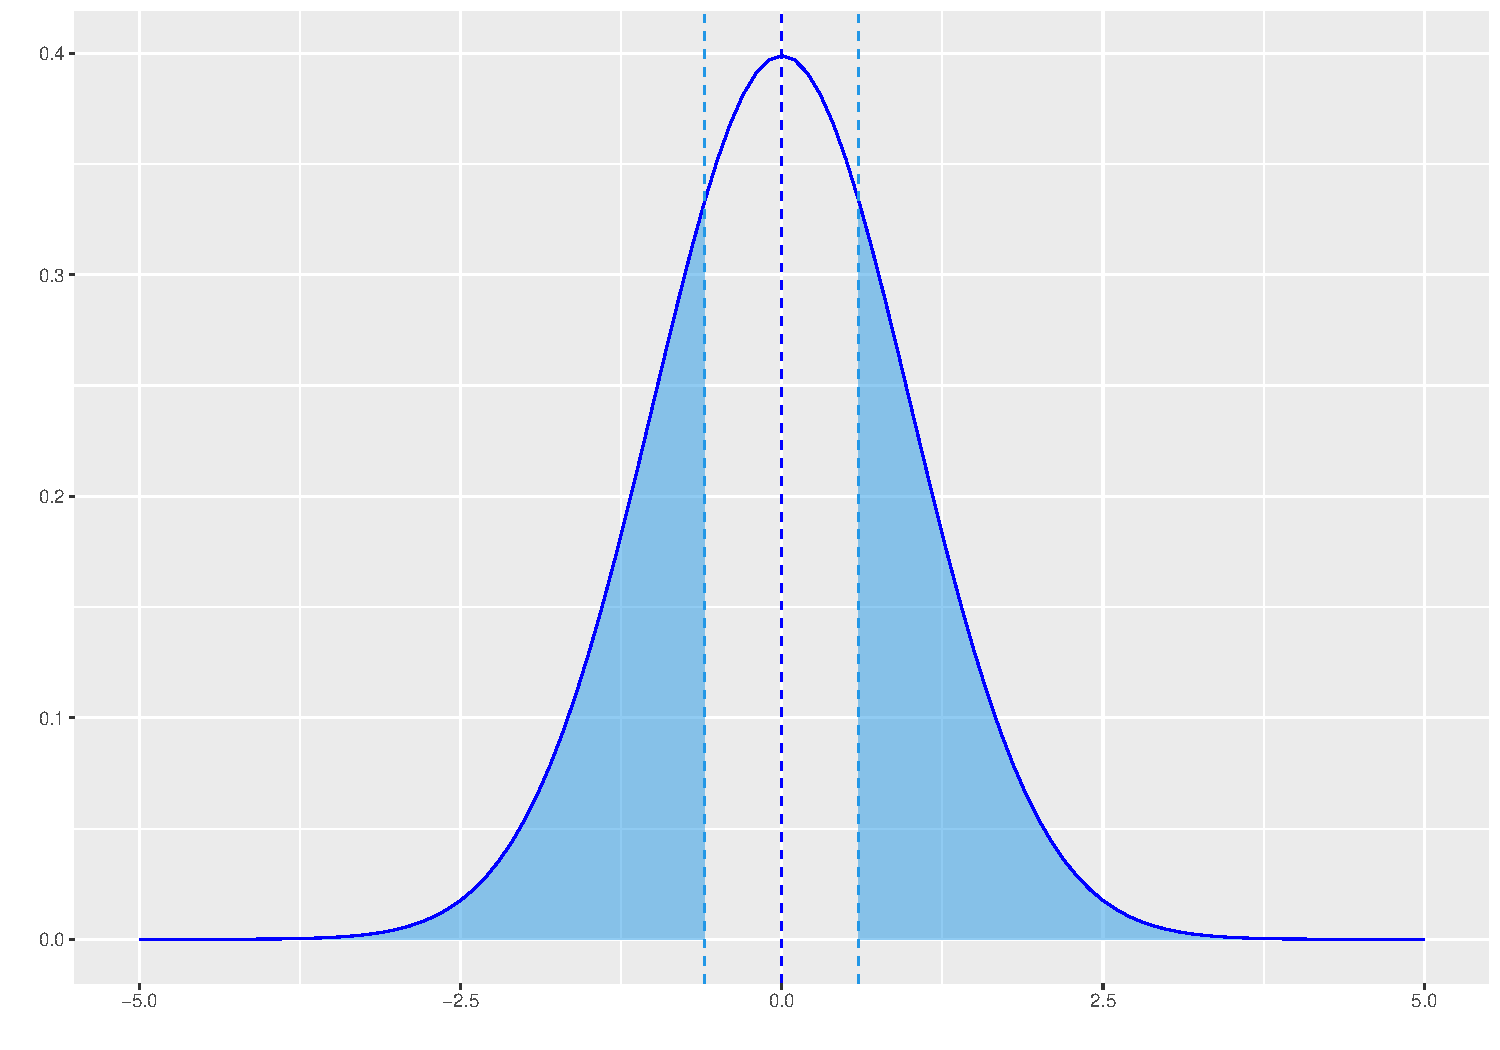
\includegraphics[width=0.8\linewidth]{ECON1013_Tutorial-4-_files/figure-beamer/unnamed-chunk-2-1} \end{center}

Looking at the statistical tables:
\(P\left(Z\leq 0.5983\right)\approx 0.7257\). Hence, \[
p-value = P(Z < -0.5983) + P(Z > 0.5983) = 2(1-0.7257) = 0.5486
\]
\end{frame}

\begin{frame}{(b) Compute the p-value associated with the test
statistics}
\protect\hypertarget{b-compute-the-p-value-associated-with-the-test-statistics-1}{}
The p-value is the probability of obtaining a value of the test
statistic \textit{as extreme as or more extreme} than the actual value
obtained when the null hypothesis is true. Thus, the p-value is the
\textit{smallest} significance level at which a null hypothesis can be
\textit{rejected}, given the observed sample statistic.

Here, the large p-value should be interpreted as evidence against the
rejection of the null hypothesis: \[
p-value = 0.5486 \Longrightarrow \text{We do not reject } H_0 \text{ at } \alpha = 0.05
\]
\end{frame}

\begin{frame}{Decision rule based on p-value}
\protect\hypertarget{decision-rule-based-on-p-value}{}
\begin{center}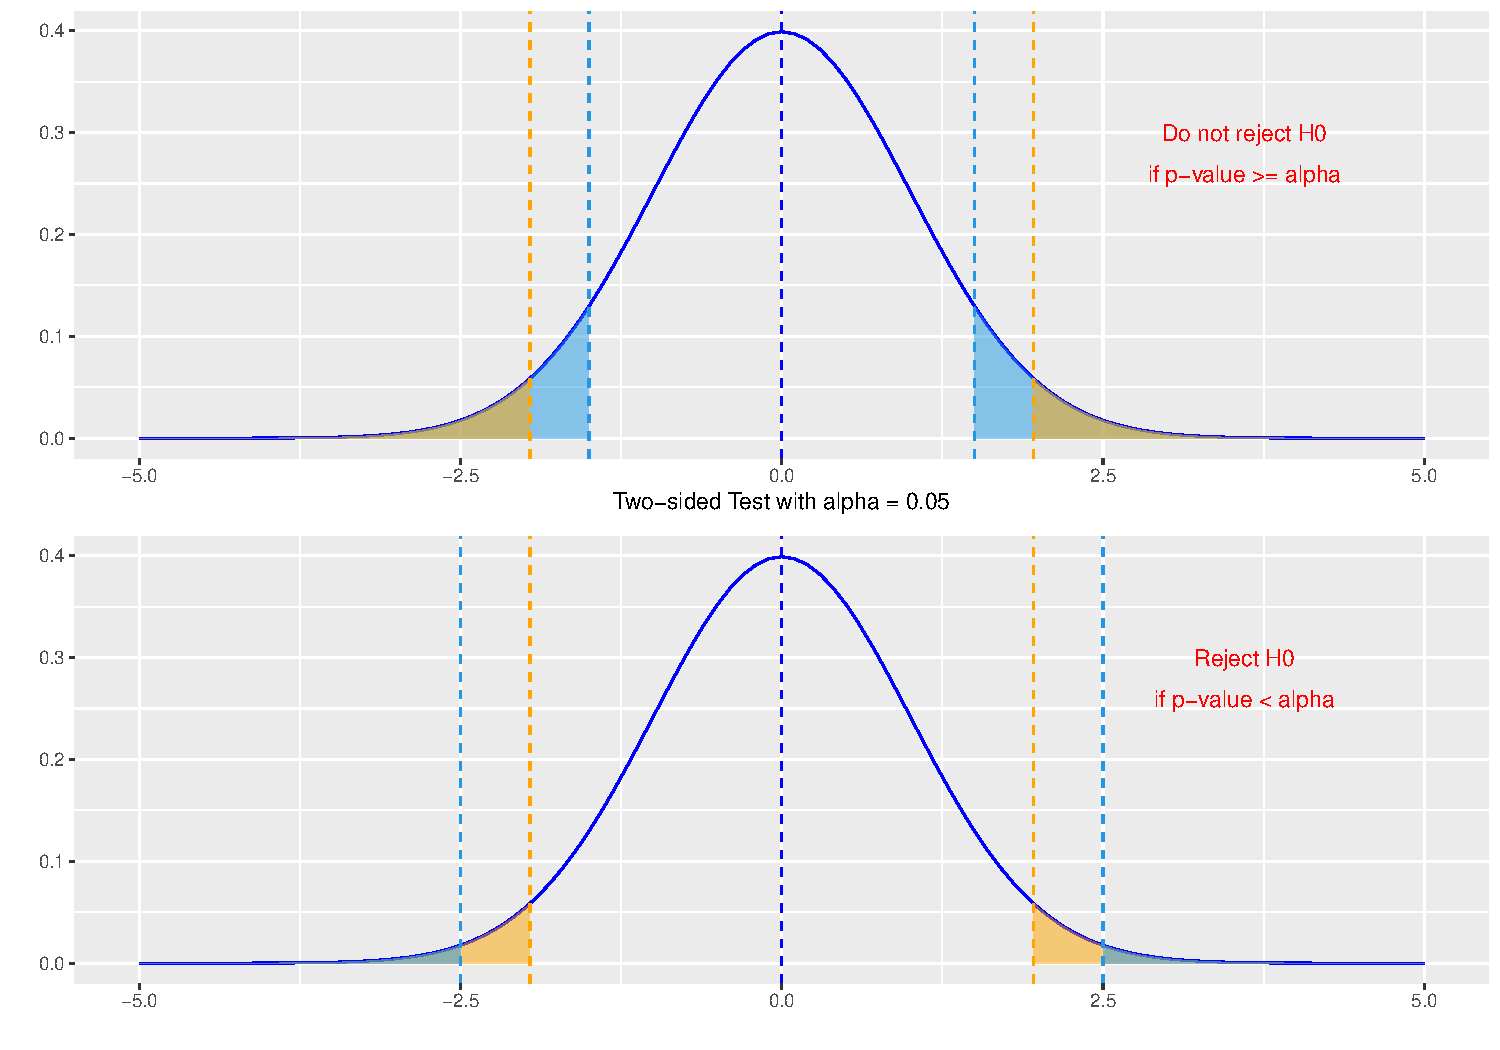
\includegraphics[width=1\linewidth]{ECON1013_Tutorial-4-_files/figure-beamer/unnamed-chunk-3-1} \end{center}
\end{frame}

\begin{frame}{Decision rule based on p-value}
\protect\hypertarget{decision-rule-based-on-p-value-1}{}
\begin{center}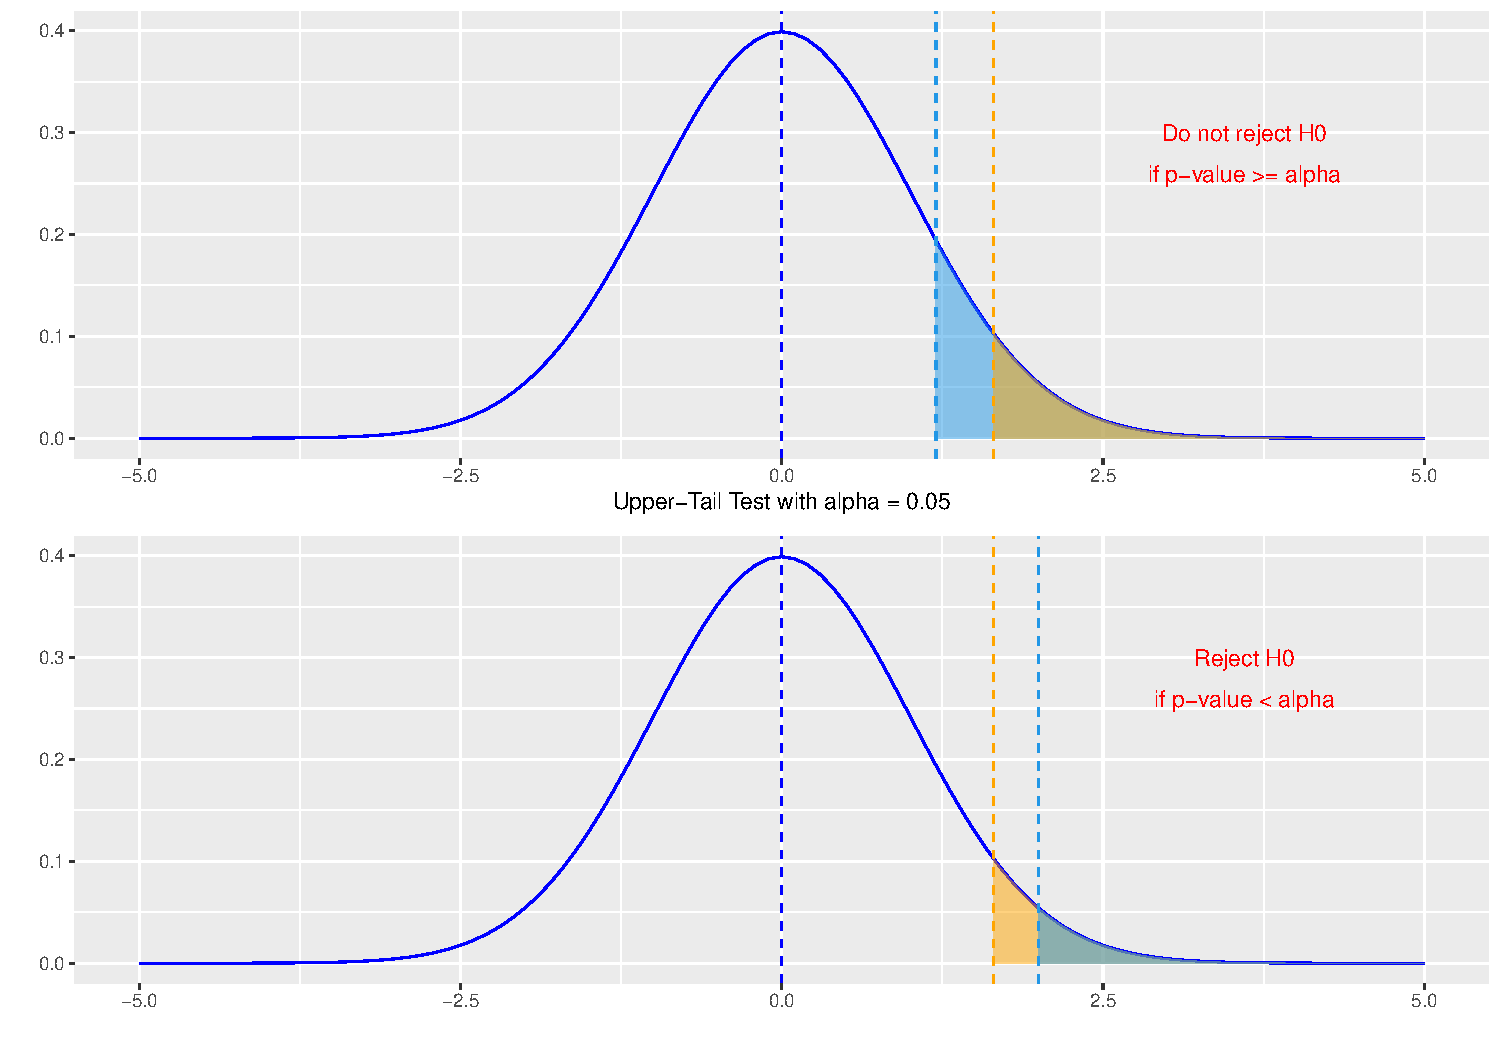
\includegraphics[width=1\linewidth]{ECON1013_Tutorial-4-_files/figure-beamer/unnamed-chunk-4-1} \end{center}
\end{frame}

\begin{frame}{Decision rule based on p-value}
\protect\hypertarget{decision-rule-based-on-p-value-2}{}
\begin{center}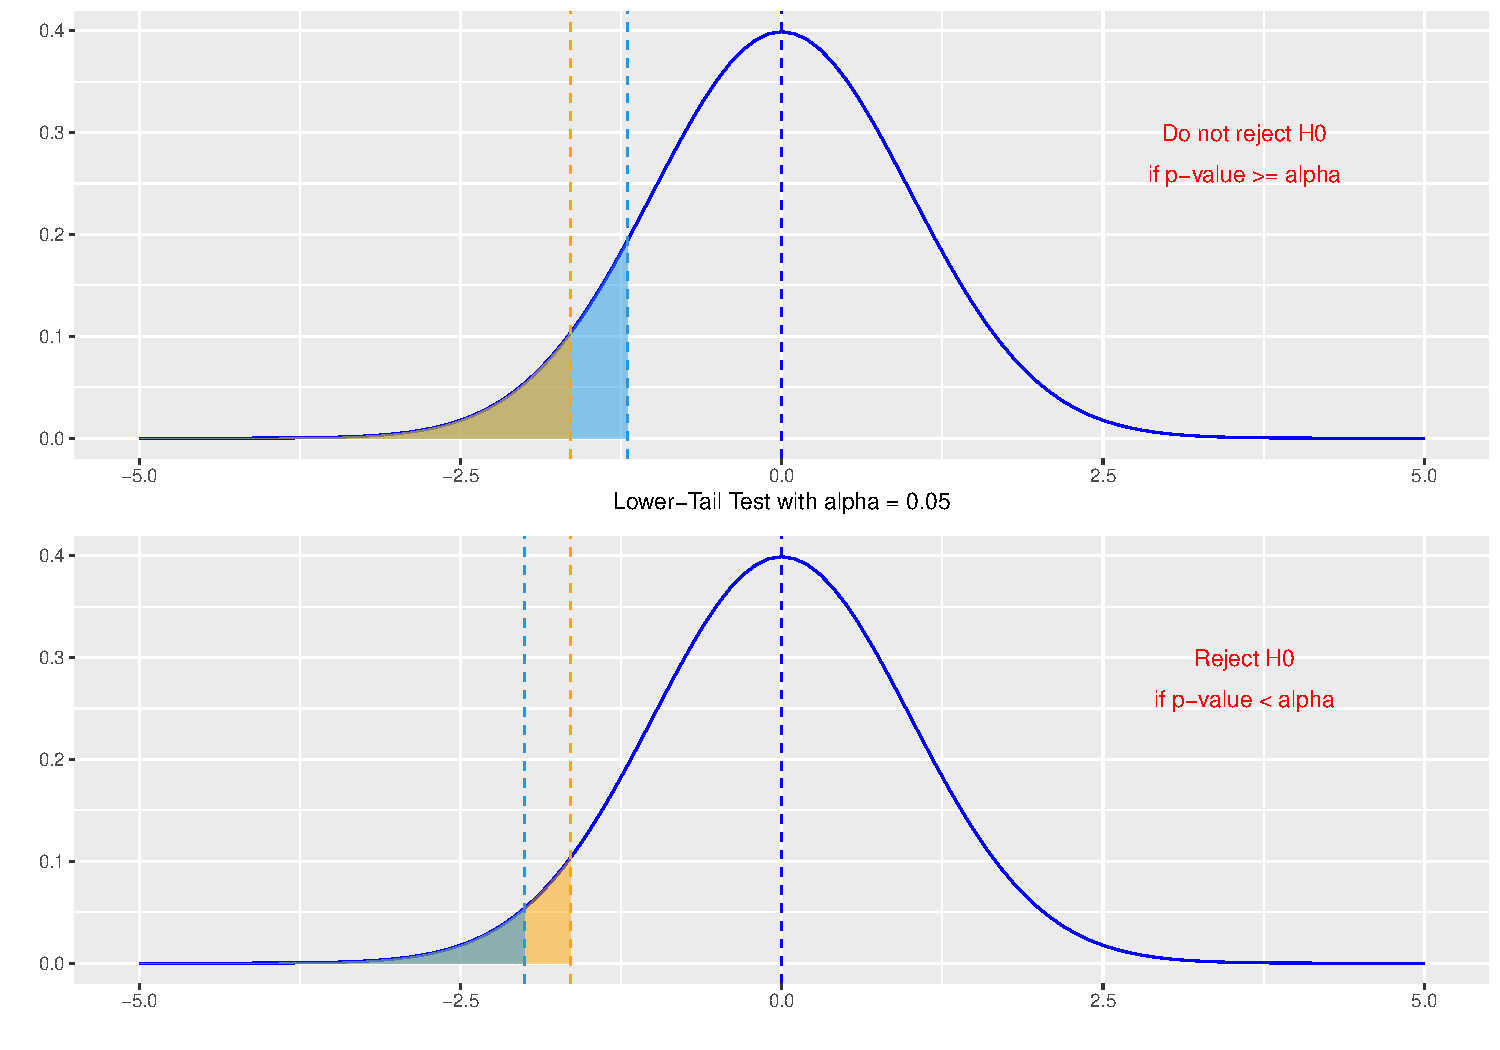
\includegraphics[width=1\linewidth]{ECON1013_Tutorial-4-_files/figure-beamer/unnamed-chunk-5-1} \end{center}
\end{frame}

\begin{frame}{Exercise 2}
\protect\hypertarget{exercise-2}{}
Supporters claim that a new windmill can generate an average of at least
800 kilowatts of power per day. Daily power generation for the windmill
is assumed to be normally distributed with a standard deviation of 120
kilowatts. A simple random sample of 100 days is taken to test this
claim against the alternative hypothesis that the true mean is less than
800 kilowatts. The claim will not be rejected if the sample mean is 776
kilowatts or more and rejected otherwise.

\begin{enumerate}
    \item [(a)] What is the probability $\alpha$ of a Type I error using the decision rule if the population mean is, in fact, 800 kilowatts per day?
    \item [(b)] What is the probability $\beta$ of a Type II error using this decision rule if the population mean is, in fact, 740 kilowatts per day?
    \item [(c)] Suppose that the same decision rule is used, but with a sample of 200 days rather than 100 days.
    \begin{enumerate}
        \item [(i)] Would the value of $\alpha$ be larger than, smaller than, or the same as that found in part (a)? Explain.
        \item [(ii)] Would the value of $\beta$ be larger than, smaller than, or the same as that found in part (b)? Explain.
    \end{enumerate}
\end{enumerate}
\end{frame}

\begin{frame}{Hypothesis Testing}
\protect\hypertarget{hypothesis-testing}{}
Denote \(\mu\) the population mean of daily power generated by the
windmill.

\begin{itemize}
    \item Null hypothesis $H_0$
        \pause
        \begin{itemize}
            \item [$\square$] $H_0$: The population mean is at least 800 kilowatts\\
                  $H_0: \mu \geq 800$
    \end{itemize}
    \vspace{1.5mm}
    \item Alternative hypothesis $H_1$
        \pause
        \begin{itemize}
            \item [$\square$] $H_1$: The population mean is less than 800 kilowatts\\
                  $H_1: \mu < 800$\\
        \end{itemize}
    \vspace{1.5mm}
    \item Decision rule
        \pause
        \begin{itemize}
            \item [$\square$] Do not reject $H_0$ if the sample mean is 776 kilowatts or more and reject $H_0$ otherwise. \\
        \end{itemize}
    \vspace{1.5mm}
\end{itemize}
\end{frame}

\begin{frame}{Hypothesis Testing}
\protect\hypertarget{hypothesis-testing-1}{}
\includegraphics[width=1\linewidth]{/Users/duongtrinh/Dropbox/GLASGOW/GTA/ECON1013/Labs/Lab 3/Power of the Test}
\end{frame}

\begin{frame}{Hypothesis Testing}
\protect\hypertarget{hypothesis-testing-2}{}
\begin{center}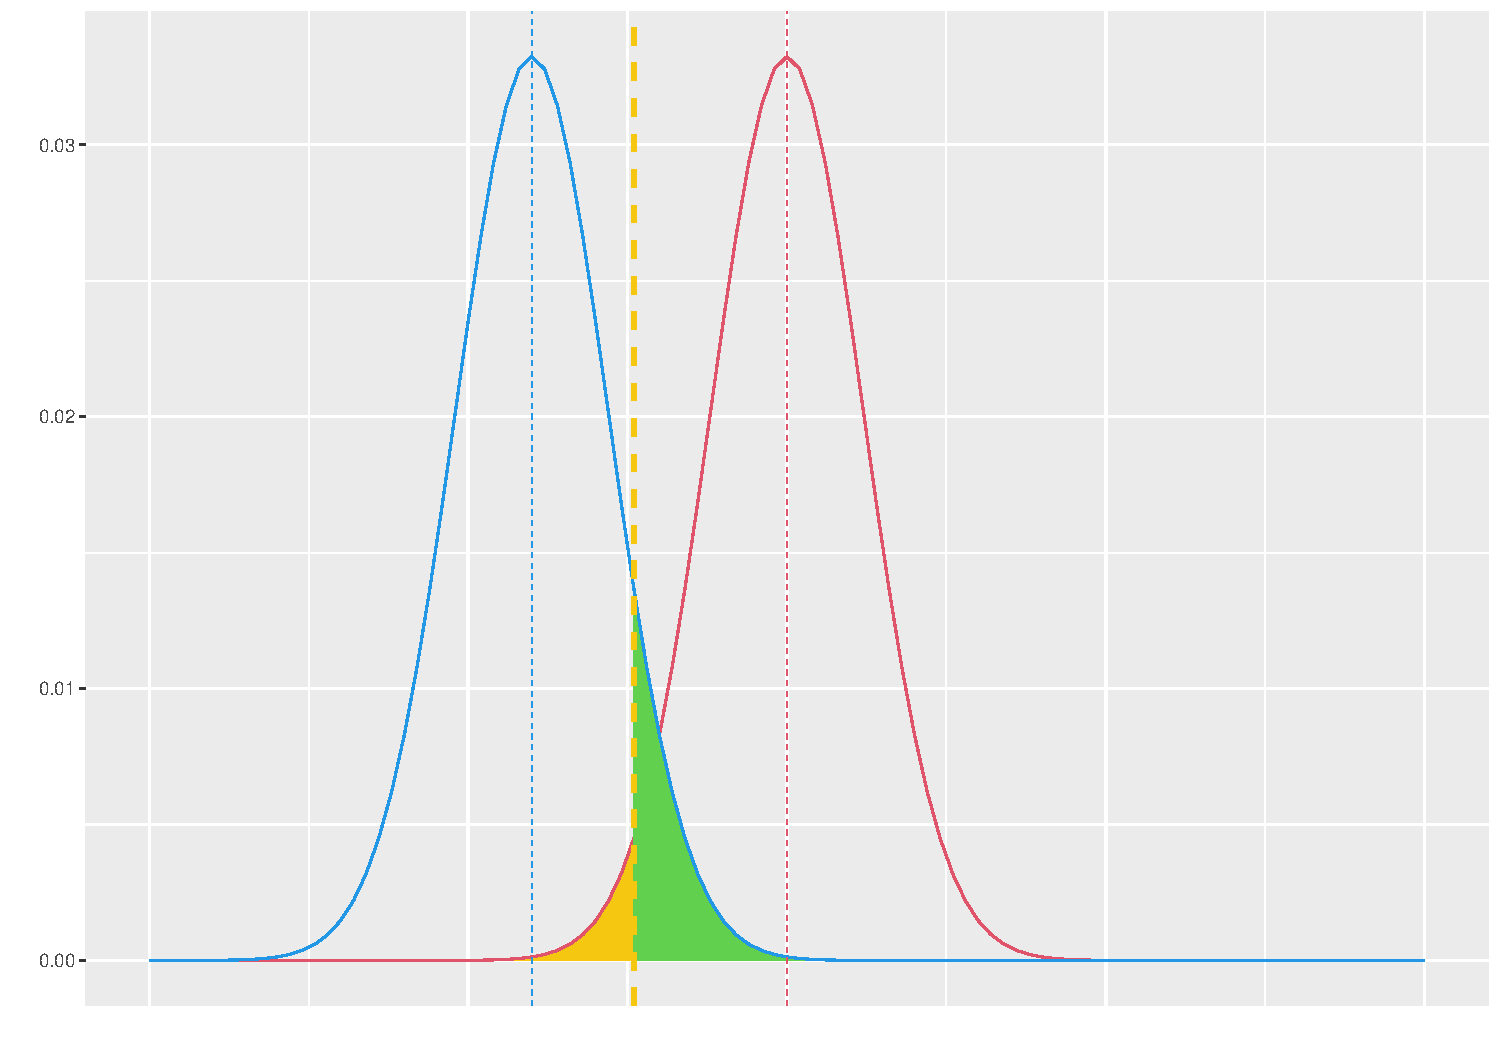
\includegraphics[width=0.8\linewidth]{ECON1013_Tutorial-4-_files/figure-beamer/unnamed-chunk-7-1} \end{center}
\end{frame}

\begin{frame}{(a) What is \(\alpha\) if \(\mu = 800\) kilowatts per
day?}
\protect\hypertarget{a-what-is-alpha-if-mu-800-kilowatts-per-day}{}
\[
\alpha = P(\textcolor{orange}{\text{ Reject } H_0} | \textcolor{red}{H_0 \text{ is true}})
\] \[
\Longleftrightarrow \alpha = P(\textcolor{orange}{\bar{X} < 776} | \textcolor{red}{\mu = 800})
\]

Under the null hypothesis \(H_0\): \[
\alpha = P\left(\frac{\bar{X}-\textcolor{red}{800}}{\sigma/\sqrt{n}} < \frac{776-\textcolor{red}{800}}{\sigma/\sqrt{n}}\right) = P\left(Z < \frac{776-\textcolor{red}{800}}{120/\sqrt{100}}\right) = P\left(Z < -2\right)
\]

where
\(Z = \frac{\bar{X}-\textcolor{red}{800}}{\sigma/\sqrt{n}} \sim N(0,1); \sigma = 120; n =100\)

\vspace{3mm}
\pause

Looking at the statistical table: \[
P\left(Z < -2\right) = 0.0228 \Longrightarrow \alpha = 0.028
\]
\end{frame}

\begin{frame}{(b) What is \(\beta\) if \(\mu = 740\) kilowatts per day?}
\protect\hypertarget{b-what-is-beta-if-mu-740-kilowatts-per-day}{}
\[
\beta = P(\textcolor{green}{\text{ Do not reject } H_0} | \textcolor{blue}{H_0 \text{ is false}})
\]

\[
\Longleftrightarrow \beta = P(\textcolor{green}{\bar{X} \geq 776} | \textcolor{blue}{\mu = 740})
\]

Under the alternative hypothesis \(H_1\): \[
\beta = P\left(\frac{\bar{X}-\textcolor{blue}{740}}{\sigma/\sqrt{n}} \geq \frac{776-\textcolor{blue}{740}}{\sigma/\sqrt{n}}\right) = P\left(Z \geq \frac{776-\textcolor{blue}{740}}{120/\sqrt{100}}\right) = P\left(Z \geq 3\right)
\] where
\(Z = \frac{\bar{X}-\textcolor{blue}{740}}{\sigma/\sqrt{n}} \sim N(0,1); \sigma = 120; n =100\)

\vspace{3mm}
\pause

Looking at the statistical table: \[
P\left(Z < 3\right) = 0.9987 \Longrightarrow \beta = 1-0.9987 = 0.013
\]
\end{frame}

\begin{frame}{(c) Same decision rule is used, but with a sample of 200
days rather than 100 days}
\protect\hypertarget{c-same-decision-rule-is-used-but-with-a-sample-of-200-days-rather-than-100-days}{}
\begin{enumerate}
        \item [(i)] Would the value of $\alpha$ be larger than, smaller than, or the same as that found in part (a)? Explain.
        
\pause 
\vspace{3mm}

$$
        \alpha = P\left(Z < \frac{776-800}{120/\textcolor{purple}{\sqrt{200}}}\right) = P\left(Z < -2{\textcolor{purple}{\sqrt{2}}}\right)
$$
become \textit{smaller}
\end{enumerate}
\end{frame}

\begin{frame}{(c) Same decision rule is used, but with a sample of 200
days rather than 100 days}
\protect\hypertarget{c-same-decision-rule-is-used-but-with-a-sample-of-200-days-rather-than-100-days-1}{}
\begin{enumerate}
        \item [(ii)] Would the value of $\beta$ be larger than, smaller than, or the same as that found in part (b)? Explain.
        
\pause 
\vspace{3mm}

$$
\beta = P\left(Z \geq \frac{776-740}{120/\textcolor{purple}{\sqrt{200}}}\right) = P\left(Z \geq 3\textcolor{purple}{\sqrt{2}}\right)
$$
become \textit{smaller}
\end{enumerate}
\end{frame}

\end{document}
